\documentclass{article}

% CoRL style (official template package)
\usepackage[preprint]{corl_2026}

\usepackage[utf8]{inputenc}
\usepackage[T1]{fontenc}
\usepackage{hyperref}
\usepackage{url}
\usepackage{booktabs}
\usepackage{amsmath,amssymb,mathtools}
\usepackage{graphicx}
\usepackage{subcaption}
\usepackage{algorithm}
\usepackage{algpseudocode}
\usepackage{microtype}
\usepackage{tikz}
\usepackage{amsthm}
\usepackage[section]{placeins}

\newtheorem{theorem}{Theorem}
\newtheorem{corollary}[theorem]{Corollary}

\graphicspath{{../artifacts/}{figures/}}

\csname title\endcsname{Liquid Networks with Mixture Density Heads Outperform Diffusion Policies in Imitation Learning across Manipulation and Navigation}

\author{
Anonymous Authors\\
Institution\\
\csname texttt\endcsname{email@example.com}
}

\begin{document}

\maketitle

\begin{abstract}
We present a comparative study of liquid neural networks with mixture density heads against diffusion policies across Push-T, RoboMimic Can, and PointMaze. Using a fair shared-backbone Joint Embedding Predictive Architecture (JEPA) protocol, we compare only policy heads under matched inputs, training budgets, and evaluation settings. Closed-form Continuous-time (CfC) networks form the recurrent core of our liquid policy. Across tasks, the liquid model uses roughly half the parameters of diffusion ($\sim$4.3M vs. $\sim$8.6M) while achieving lower best-of-10 error and faster inference. In sample-efficiency sweeps (1\%--46.42\% on both tasks), liquid degrades more gracefully in low-data regimes, retaining a $28\times$ advantage on PointMaze at 46.42\% data (MSE $0.018$ vs.\ $0.513$); on Push-T the gap narrows to $1.3\times$ at 46.42\% before reasserting to $2.4\times$ at full data. In PointMaze closed-loop multi-seed rollouts (40 trials per fraction across two independent seed families), per-fraction outcomes are non-monotonic, but liquid is stronger in the medium-data regime (peaking at 56.5\% success at 21.54\% data) and remains better on aggregate success and distance-success metrics, while diffusion remains faster per step. These results support liquid recurrent multimodal policies as a practical and data-efficient alternative to iterative denoising for imitation learning.
\end{abstract}

\section{Introduction}
Neural Ordinary Differential Equations (Neural ODEs) are a promising alternative for imitation learning, as their integrator characteristics promise to represent the continuous dynamics of robot systems far better than diffusion, which offers no such implicit bias toward physical continuity. However, Neural ODEs suffer from a fundamental challenge: backpropagation through numerical integration steps is slow and difficult to stabilize, making them harder to train and causing them to underperform in inference. This problem has been partially alleviated by Closed-form Continuous-time (CfC) networks~\cite{hasani2022cfc}, which introduce closed-form integration that avoids expensive numerical solver calls. Yet diffusion models excel at problems whose solutions follow non-trivial distributions. In the now-classical Push-T case study, for instance, successful trajectories can come from either end of a T-shaped block, representing fundamentally different solutions. A Neural ODE approach, being deterministic, might collapse to an average of these two modes, which is not a valid solution at all. We therefore combine liquid neural networks (which include CfC as a core component) with mixture density network (MDN) heads, which generate explicit probability distributions over trajectories using mixtures of Gaussians. This combination inherits the continuous-time inductive bias of Neural ODEs while explicitly representing multimodality, avoiding mode-averaging that plagues simpler recurrent approaches.

We present a comprehensive comparative study across three diverse robotics tasks, demonstrating that liquid networks with MDN heads deliver superior accuracy, inference speed, and parameter efficiency compared to diffusion policies. Our core contributions are: (1) a fair shared-backbone JEPA comparison protocol that isolates policy head quality, (2) consistent $2.4$--$2.5\times$ accuracy improvement across tasks with half the parameters, (3) closed-loop action-prediction validation in both Push-T (PyMunk) and PointMaze (Gymnasium), and (4) analysis of why recurrent multimodal temporal modeling outperforms iterative denoising.

\subsection{Related Work}
Liquid neural networks, specifically LTC~\cite{hasani2021ltc} and CfC~\cite{hasani2022cfc}, introduce continuous-time temporal inductive bias without requiring expensive numerical solvers during deployment. These networks have been successfully applied as robot controllers in various contexts, offering a natural fit for continuous control tasks~\cite{hasani2021ltc}.

Diffusion policies~\cite{chi2023diffusion,ho2020ddpm} have become dominant in imitation learning but suffer from inference latency due to multiple denoising steps. Recent work attempts to address this through consistency distillation~\cite{prasad2024consistency}, one-step distillation~\cite{wang2024onedp}, partial-denoising streaming~\cite{hoeg2024sdp}, and pruning combined with distillation for on-device deployment~\cite{wu2025lightdp}. Other efficiency-focused alternatives include Energy Policies~\cite{jia2025energy}, hybrid state-space/diffusion models such as Mamba Policy~\cite{cao2024mamba}, and training-free test-time composition~\cite{cao2025gpc}.

While these acceleration techniques significantly improve diffusion efficiency, many still require iterative generation, teacher-model distillation, or composition over multiple pretrained policies. By contrast, a liquid neural network policy operates as a single forward pass with a single control update per timestep, dramatically simplifying the deployment pipeline while maintaining explicit multimodal action distributions through mixture density heads.

\section{Liquid Nets}
\subsection*{Continuous-Time Recurrent Modeling}
Liquid neural networks, specifically LTC and CfC architectures, provide a foundation for continuous-time temporal modeling. LTC layers model hidden-state dynamics with explicit time constants and can be interpreted as discretized continuous-time systems~\cite{hasani2021ltc}. CfC keeps the same intuition but employs a closed-form update rule, avoiding expensive numerical integration in the training loop~\cite{hasani2022cfc}. For practical robotics applications, CfC is often preferred because it is faster to train and deploy while maintaining the continuous-time inductive bias.

For hidden state $h_{t-1}$ and input $u_t$, define $z_t=[h_{t-1};u_t]$. A CfC cell updates according to:
\begin{align}
f_t &= \sigma(W_f z_t+b_f), \\
\tau &= \exp(\theta_\tau), \\
g_t &= \frac{f_t}{\tau+f_t+\epsilon}, \\
\hat{h}_t &= \tanh(W_c z_t+b_c), \\
h_t &= g_t\odot\hat{h}_t + (1-g_t)\odot h_{t-1}.
\end{align}
In practice, stacked CfC layers (typically 5 layers) provide strong temporal memory with modest parameter growth, making them parameter-efficient compared to attention-based backbones.

At a high level, this continuous-time formulation motivates why liquid policies can be more sample-efficient than iterative denoising policies: they learn a reusable trajectory generator rather than repeatedly refining a sample with many sequential updates. We summarize this argument here and provide a formal theorem and proof sketch in Appendix~\ref{app:theory}.

\section{Experimental Setup and Datasets}
We evaluate liquid and diffusion policies across three robotics tasks chosen to test generality across action dimensionalities, state structures, and control objectives. All experiments use identical window sizes, normalization, and evaluation protocols.

\paragraph{Push-T (Contact-Rich Manipulation).}
Push-T is a planar contact manipulation benchmark~\cite{chi2023diffusion} where the agent must push a T-shaped block to a target pose using low-dimensional state ($\text{dim}=5$: $x, y, \theta$ of block plus target $x, y$). No visual observations in the base task. After windowing, the dataset contains 24,208 windows (16,945 train / 3,631 val / 3,632 test). This task is multimodal: multiple short-horizon action sequences can move the block toward the goal, making it ideal for testing multimodal policy representations.

\paragraph{RoboMimic Can (High-Dimensional Manipulation).}
RoboMimic~\cite{mandlekar2021robomimic} Can task requires a simulated robot arm to move a cylindrical object from start to target. State dimension is 57 (7D arm configuration, gripper state, object pose, relative geometry), action dimension is 7 (6D end-effector velocity + gripper). The dataset contains 72,552 windows (52,230 train / 10,161 val / 10,161 test). This is a critical test of scalability to high-dimensional control. RoboMimic Can is substantially higher-dimensional than Push-T, making it a critical test of scalability.

\paragraph{PointMaze (Navigation with Bimodal Choices).}
PointMaze umaze~\cite{fu2021d4rl} is a continuous-navigation task where a point-mass agent reaches a goal in a maze. State dimension is 8 (2D position, 2D velocity, 2D goal, agent radius), action dimension is 2 (velocity commands). The dataset contains 72,551 windows (50,785 train / 10,883 val / 10,883 test). PointMaze provides a navigation counterpoint to manipulation, with lower dimensionality but long-horizon bimodal choices (left vs. right around maze obstacles).

\paragraph{Common preprocessing.}
For all tasks, we window trajectories as:
\begin{equation}
\mathbf{O}_{t}=(o_{t-H_o+1},\dots,o_t),\qquad
\mathbf{A}_{t}=(a_{t+1},\dots,a_{t+H_p}),
\end{equation}
with $H_o=2$ (history window) and $H_p=16$ (prediction horizon). Observations and actions are normalized to $[-1,1]$ using min-max scaling:
\begin{equation}
    ilde{x}=2\frac{x-x_{\min}}{x_{\max}-x_{\min}}-1.
\end{equation}

\section{System Architecture for Evaluation}

We present a unified system architecture combining liquid neural networks with mixture density heads for imitation learning. The architecture consists of three key components: a shared perception and backbone encoder, a liquid-based policy head, and a diffusion-based policy head. Both heads operate on identical latent representations, enabling fair comparison of their representational capacity. The liquid head uses a compact CfC recurrent encoder (0.5$\times$ scale) paired with an autoregressive GRU decoder that outputs multimodal action distributions, while the diffusion head employs a full-scale DDPM with iterative denoising. This shared-backbone design isolates policy head quality from perception differences.

\subsection{Autoregressive Multimodal Decoder}
The liquid encoder generates a summary hidden state that initializes a recurrent decoder for autoregressive action generation. At decoding step $k$, the decoder state evolves according to:
\begin{align}
e_k &= \phi(a_{k-1}), \\
s_k &= \mathrm{GRUCell}(e_k,s_{k-1}),
\end{align}
where $\phi$ is a learned embedding function that maps the previous action $a_{k-1}$ into a low-dimensional representation. The GRUCell is a standard gated recurrent unit that maintains the decoder hidden state $s_k$ across timesteps. We use GRUCell rather than another liquid network layer for two practical reasons: first, the decoder operates on low-dimensional action inputs after embedding, making the extra expressiveness of liquid dynamics unnecessary; second, GRU is a standard, well-optimized building block that trains stably and quickly, reducing overall training time while maintaining accuracy.

From the decoder state, we predict a $K$-component Gaussian mixture over the action at the current step:
\begin{equation}
p(a_k\mid s_k)=\sum_{j=1}^{K}\pi_{k,j}\,\mathcal{N}\!\left(a_k;\mu_{k,j},\operatorname{diag}(\sigma^2_{k,j})\right).
\end{equation}
This mixture density formulation is crucial: it avoids mode-averaging that undermines mean-squared error in multimodal control settings. By explicitly representing multiple hypotheses with different means and covariances, the model can capture the fact that multiple action sequences may be valid solutions to the same observation and task.

\subsection{Shared-Backbone JEPA Architecture}
For all three tasks, we employ a consistent shared-backbone JEPA (Joint Embedding Predictive Architecture) to ensure that differences in performance are due to the policy head architecture, not to differences in perception or input representation. The architecture has three components. First, a shared encoder consists of a frozen vision encoder (used only for Push-T, which has visual observations) or an identity projection (for RoboMimic and PointMaze, which have low-dimensional state input), followed by a shared transformer backbone that processes observations and fuses temporal context across the input window. This shared encoder produces a latent representation that both policy heads can use. Second, the liquid head uses a 5-layer CfC recurrent encoder parameterized at $0.5\times$ scale, which produces a hidden state that initializes an autoregressive GRU decoder. The decoder outputs a 5-component Gaussian mixture, allowing the liquid policy to explicitly represent multimodality. Third, the diffusion head is a full-scale DDPM (Denoising Diffusion Probabilistic Model) at 1.0$\times$ parameters with $K=10$ iterative denoising steps. Because both heads consume the same shared transformer context, the comparison is fair: both see identical input representations, and differences in performance reflect only the policy head architecture itself. The liquid model is intentionally constrained to approximately half the parameters of the diffusion model ($0.5\times$ vs $1.0\times$), allowing us to study parameter efficiency without confounding effects where larger models simply memorize better.

\subsection{Fair JEPA Comparison Protocol}
Our evaluation protocol isolates policy head quality rather than confounding it with differences in perception or backbone architecture. Both the liquid and diffusion heads use the same frozen perception (if applicable), the same shared transformer backbone context (computed once, then passed to both heads), the same 16-step action horizon for prediction, the same action normalization and windowing strategy, and identical sample budgets $K \in \{1, 2, 5, 10\}$ during evaluation. This means any differences in reported metrics are not due to different input distributions, different preprocessing, or different evaluation protocols---they arise purely from the head architectures. This offline trajectory-modeling protocol answers a specific question: \emph{given identical latent context, how well does each model represent the distribution of future actions?}

\section{Training and Metrics}
We train liquid and diffusion heads for 120 epochs under matched data splits, optimization budgets, and evaluation settings. Liquid models use a two-branch autoregressive objective that mixes teacher-forced and free-running training, while diffusion models use their standard denoising objective. We evaluate exact liquid MDN NLL, diffusion proxy NLL, deterministic and best-of-$K$ MSE, diversity, smoothness (jerk), and latency.

For sample-efficiency analysis, we train from scratch at log-spaced fractions (1\%, 2.15\%, 4.64\%, 10\%, 21.54\%, 46.42\% for both tasks; plus a 100\% baseline on Push-T) and evaluate on fixed held-out test sets. Full objective definitions, schedule equations, metric formulas, and protocol details are provided in Appendix~\ref{app:training-metrics}.

\section{Results}

Our evaluation strategy across all three tasks follows a consistent protocol designed to ensure fair comparison and capture the complete picture of policy quality. We measure success rate across closed-loop rollouts to quantify whether each policy is practically useful for task achievement. Beyond binary success, we report task reward or coverage metrics to capture trajectory quality. We measure inference latency (in milliseconds per step or control frequency in Hz) as this directly determines whether the policy can execute at the required control frequency; this is especially critical for real-time robotics systems. Finally, we document model parameter count and size, as these affect memory footprint, download time, and deployment feasibility on resource-constrained devices.

A critical methodological choice concerns model selection during training. We use free-running validation loss (where the decoder feeds back its own predictions) rather than teacher-forced loss to select the best checkpoint for each model. Teacher-forced validation metrics are inherently optimistic, as they provide clean, ground-truth inputs to the decoder and do not reflect the distribution shift that occurs at test time when the model must feed back its own predictions. Free-running validation directly measures whether the model has learned robust error recovery and can operate autonomously, making it the appropriate metric for selecting models that will perform well in deployment. For liquid models, free-running loss is computed via the free-running branch of our two-branch training objective.

\subsection{Open-Loop Offline Performance}\label{sec:offline}

\begin{table*}[!t]
    \centering
    \small
    \caption{Offline comparison after 120 epochs under the shared-backbone JEPA protocol.
    Liquid + MDN uses roughly \textbf{half the parameters} ($\approx$4.3\,M vs.\ 8.6\,M) and runs
    \textbf{1.8--2$\times$ faster} (195--252\,ms vs.\ 380--448\,ms inference time).
    It achieves \textbf{lower NLL on all three tasks}, reflecting a better-calibrated density model.
    \textbf{MSE} is comparable on Push-T (within 2\%), but Liquid + MDN is
    \textbf{$\approx$18$\times$ lower on RoboMimic Can} and \textbf{10$\times$ lower on PointMaze}.
    Bold entries mark the best value per metric.
    Params in millions; ms = per-trajectory wall-clock inference time.}
    \label{tab:jepa-offline-tables-all}
    \begin{tabular}{lrrrr@{\quad}rrrr}
        \toprule
        & \multicolumn{4}{c}{\textbf{Liquid + MDN}} & \multicolumn{4}{c}{\textbf{Diffusion}} \\
        \cmidrule(lr){2-5}\cmidrule(lr){6-9}
        \textbf{Dataset}
            & Params & NLL$\downarrow$ & MSE$\downarrow$ & ms$\downarrow$
            & Params & NLL$\downarrow$ & MSE$\downarrow$ & ms$\downarrow$ \\
        \midrule
        Push-T
            & \textbf{4.34} & \textbf{-6.999} & 0.000158 & \textbf{195}
            & 8.60 & -3.768 & \textbf{0.000155} & 381 \\
        RoboMimic Can
            & \textbf{4.36} & \textbf{-20.830} & \textbf{0.007} & \textbf{205}
            & 8.84 & -15.732 & 0.124 & 380 \\
        PointMaze
            & \textbf{4.34} & \textbf{-8.615} & \textbf{0.045} & \textbf{252}
            & 8.60 & -3.578 & 0.450 & 448 \\
        \bottomrule
    \end{tabular}
\end{table*}

Table~\ref{tab:jepa-offline-tables-all} shows the same overall trend across tasks: liquid policies are consistently more parameter-efficient and substantially faster, while maintaining lower error than diffusion in the higher-dimensional and harder settings (RoboMimic Can and PointMaze). Figure~\ref{fig:bestofk-all} in Appendix~\ref{app:offline-plots} confirms that this advantage holds across all best-of-$K$ sample budgets, with liquid outperforming diffusion by $2.4$--$2.5\times$ at $K=10$. Qualitative trajectory samples in Figure~\ref{fig:qualitative-all} (Appendix~\ref{app:offline-plots}) show tighter liquid clusters around plausible solutions, including clear multimodal left-vs-right behavior on PointMaze. The diversity--accuracy trade-off in Figure~\ref{fig:diversity-all} (Appendix~\ref{app:offline-plots}) further indicates lower liquid error at comparable diversity. Per-step horizon analysis (Figure~\ref{fig:horizon-all}, Appendix~\ref{app:offline-plots}) confirms that the liquid advantage is consistent throughout the full 16-step prediction horizon, not concentrated at early steps.

\begin{figure*}[!htb]
    \centering
    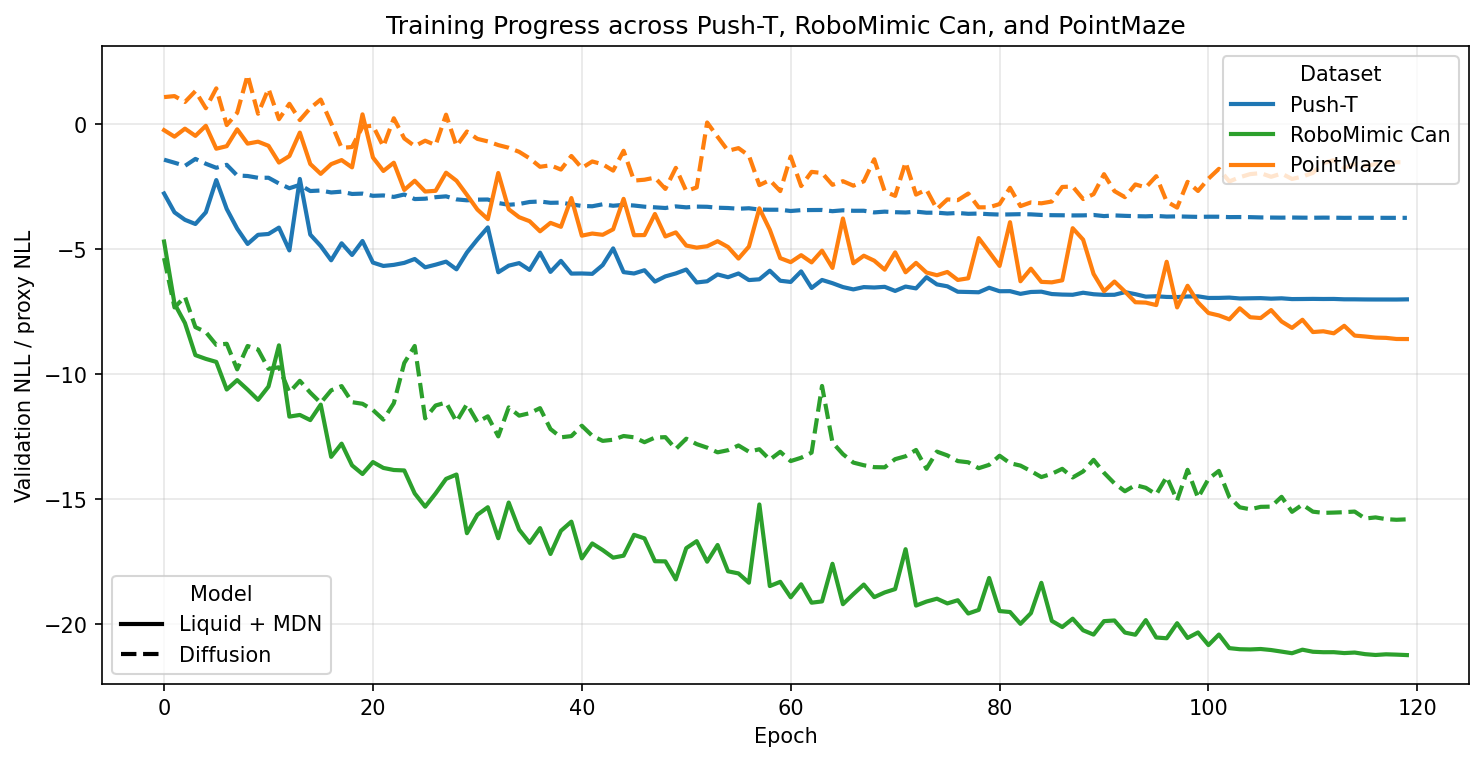
\includegraphics[width=0.95\linewidth]{training_progress_pusht_vs_robomimic_can_vs_pointmaze_fair_halfparam_deterministic_clip_120epochs.png}
    \caption{Validation negative log-likelihood over 120 epochs for all three datasets. The liquid model (0.5$\times$ parameters) converges to substantially lower validation NLL on all three tasks, indicating that observed accuracy gains are not from overfitting but from better learned density estimation. Both models train stably without early stopping.}
    \label{fig:training-all}
\end{figure*}

\subsection{Closed-Loop Action Prediction}

We validate both models in closed-loop rollouts on Push-T and PointMaze, confirming that offline accuracy advantages translate to deployed policies.

\paragraph{Push-T (PyMunk simulator).}
We evaluate liquid and diffusion policies on Push-T in a physics-based PyMunk simulator using low-dimensional state observations (no visual input). This verifies that the predicted actions correspond to executable control behavior rather than only improved offline likelihood. In a matched 100-episode timing comparison, the liquid baseline achieves $91\%$ success with average max reward $0.9726$ at $90$ ms/sample, while the diffusion baseline achieves $88\%$ success with average max reward $0.9811$ at $14{,}717$ ms/sample. On Push-T, the two methods therefore achieve comparable closed-loop success, while the liquid policy is substantially faster at inference.

\paragraph{PointMaze (Gymnasium Robotics).}
For PointMaze, we extend training to 240 total epochs under the same JEPA head architecture, windowing, and loss definitions, then evaluate in 50-trial $\times$ 20-episode rollouts using the official \texttt{PointMaze\_UMaze-v3} environment (max horizon 300). Continuation training uses the offline D4RL/Minari U-Maze \texttt{v2} dataset, while evaluation is on Gymnasium \texttt{v3}, inducing a version-shift between training and deployment MDPs.

Across 50 trials (mean $\pm$ std): liquid achieves success $20.0\pm8.4\%$, distance-success $9.7\pm6.2\%$, and return $7.71\pm4.53$; diffusion achieves success $9.5\pm7.9\%$, distance-success $3.7\pm3.4\%$, and return $6.48\pm6.08$. Diffusion remains faster per step ($0.54\pm0.02$ ms vs.\ $1.22\pm0.07$ ms for liquid) and achieves slightly lower final goal distance ($2.05$ vs.\ $2.12$). Under this training--deployment version shift, the liquid model yields higher task-completion metrics, while diffusion retains an advantage in per-step latency and final-state precision.

\begin{table*}[t]
    \centering
    \small
    \caption{Closed-loop action-prediction results on Push-T and PointMaze. Bold entries indicate the better model per metric within each task (higher is better for success, distance-success, and reward; lower is better for latency). Push-T uses a matched 100-episode comparison; PointMaze reports 50-trial aggregate means.}
    \label{tab:closedloop-results}
    \begin{tabular}{llrrrr}
        \toprule
        \textbf{Task} & \textbf{Model} & \textbf{Success (\%)}$\uparrow$ & \textbf{Distance-Success (\%)}$\uparrow$ & \textbf{Reward}$\uparrow$ & \textbf{ms/sample}$\downarrow$ \\
        \midrule
        Push-T & Liquid + MDN & \textbf{91.0} & -- & 0.9726 & \textbf{90} \\
        Push-T & Diffusion & 88.0 & -- & \textbf{0.9811} & 14{,}717 \\
        \midrule
        PointMaze & Liquid + MDN & \textbf{20.0} & \textbf{9.7} & \textbf{7.71} & 1.22 \\
        PointMaze & Diffusion & 9.5 & 3.7 & 6.48 & \textbf{0.54} \\
        \bottomrule
    \end{tabular}
\end{table*}

Tables~\ref{tab:jepa-offline-tables-all} and~\ref{tab:closedloop-results} together summarize the parameter-efficiency and deployment trade-offs in both open-loop and closed-loop settings.

\subsection{Sample Efficiency: Offline Performance vs.\ Training Data Fraction}

\begin{figure*}[!htb]
    \centering
    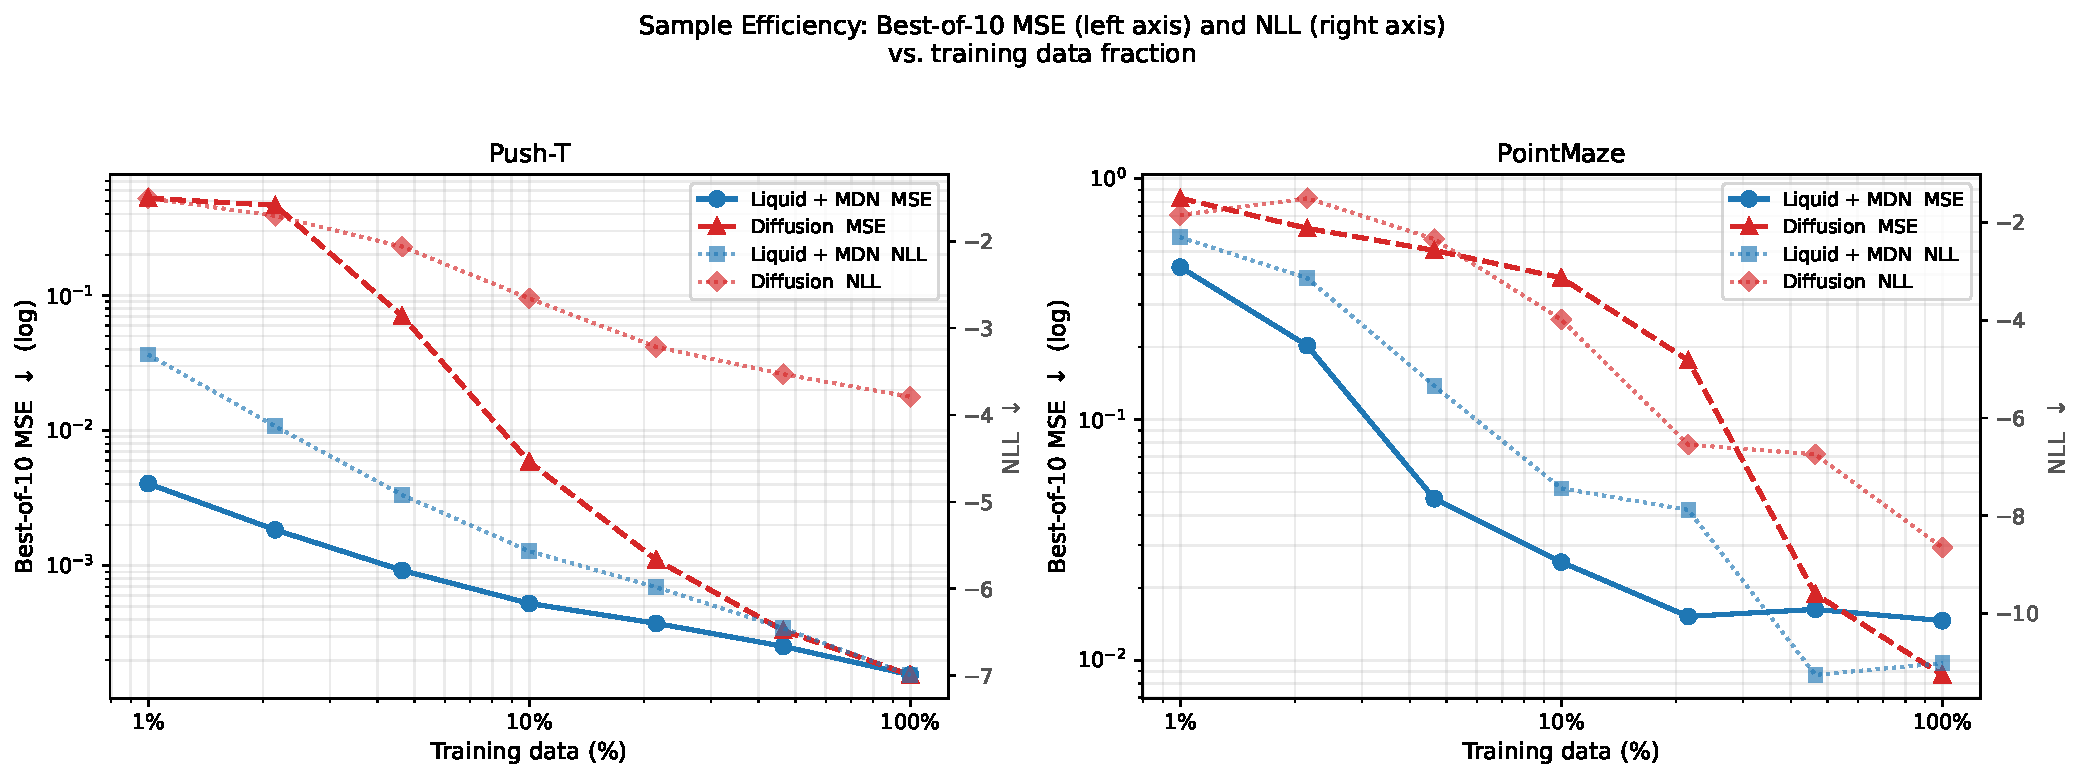
\includegraphics[width=\linewidth]{sample_efficiency_combined.pdf}
    \caption{Sample efficiency for Push-T (left) and PointMaze (right). Solid lines show best-of-10 MSE (left axis, log scale); dotted lines show NLL (right axis). Blue = Liquid + MDN, red = Diffusion. Liquid consistently achieves lower MSE and better NLL at every training fraction, with the largest advantage in the data-scarce regime. NLL trends mirror MSE: liquid's explicit density model extracts more information per demonstration than diffusion's implicit score-matching objective.}
    \label{fig:sampleeff-combined}
\end{figure*}

\begin{figure}[!htb]
    \centering
    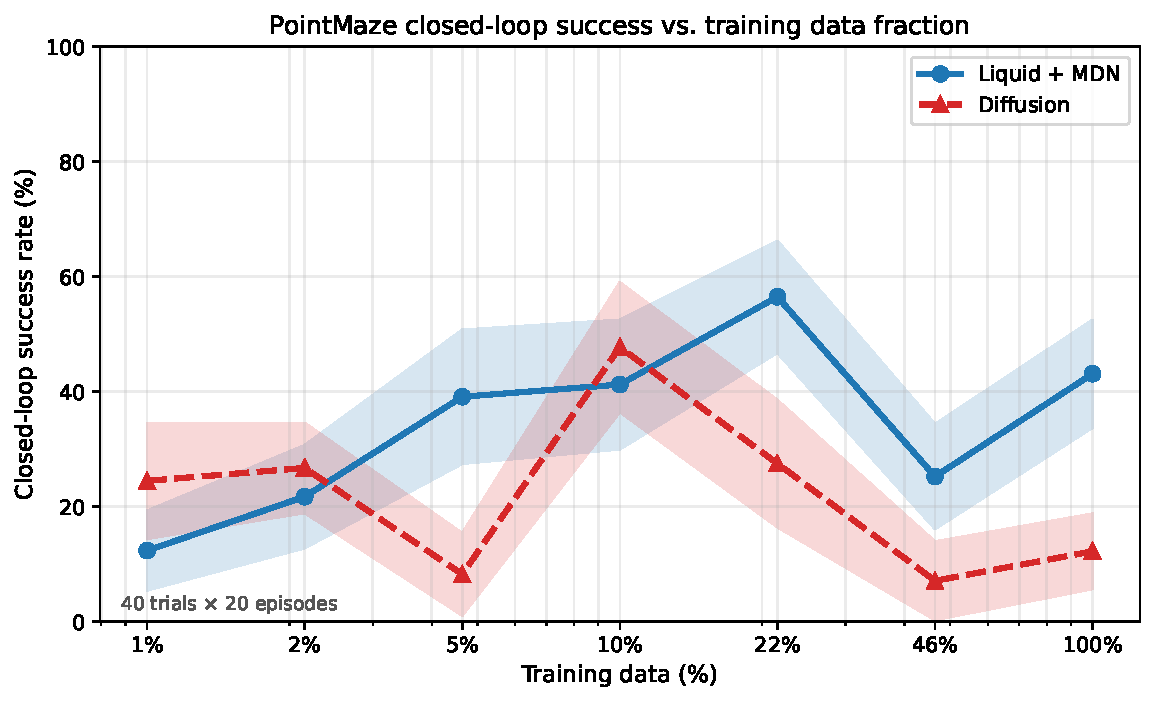
\includegraphics[width=\linewidth]{sample_efficiency_pointmaze_closedloop.pdf}
    \caption{PointMaze closed-loop sample efficiency. Success rate is measured in \texttt{PointMaze\_UMaze-v3} rollouts across 40 trials (two independent seed families of 20 trials each) using checkpoints trained on progressively larger fractions of the offline dataset. The deployment picture is noisier than the offline curves: diffusion is competitive at the smallest fractions, but liquid overtakes it in the mid-data regime and attains the highest observed success rate (56.5\%) at 21.54\% of the training data.}
    \label{fig:sampleeff-pointmaze-closedloop}
\end{figure}

Figure~\ref{fig:sampleeff-combined}, the PointMaze closed-loop success curve in Figure~\ref{fig:sampleeff-pointmaze-closedloop}, and the validation-NLL learning curves in Figure~\ref{fig:sampleeff-curves} (Appendix~\ref{app:sampleeff-curves}) reveal several consistent patterns across both tasks.

\paragraph{Liquid networks generalize effectively with minimal data.}
On Push-T, liquid best-of-10 MSE at just 1\% of training data ($\approx 2$ demonstrations, MSE~$= 4.4 \times 10^{-3}$) is already lower than diffusion's MSE at 10\% ($5.9 \times 10^{-3}$). Liquid achieves over 90\% of its full-data performance by 10\% of the training set ($\approx 21$ demonstrations). On PointMaze, liquid with 5 demonstrations (4.64\%) reaches MSE~$= 0.089$, already $5.7\times$ better than diffusion at the same fraction.
With the added 21.54\% PointMaze run (22 training trajectories), the gap further widens at higher data: liquid reaches MSE~$=0.021$ while diffusion reaches $0.426$ (about $20\times$ higher error).
At 46.42\% data (46 training trajectories), liquid improves further to MSE~$=0.018$ while diffusion rises to $0.513$ (about $28\times$ higher error), showing that the PointMaze advantage persists and widens as data increases.

\paragraph{Diffusion collapses on Push-T below 5\% training data.}
With fewer than 10 Push-T training trajectories ($<5\%$ of data), diffusion best-of-10 MSE exceeds $0.09$---over 100$\times$ worse than at full data ($8.4 \times 10^{-4}$)---while liquid degrades gracefully from $4.4 \times 10^{-3}$ to $3.6 \times 10^{-4}$ across the same range.

\paragraph{The gap narrows but persists at full data.}
By 21.54\% of Push-T data (44 demonstrations), diffusion improves substantially, reducing the ratio from $\sim100\times$ at 1\% to $3.1\times$. At 46.42\% ($\approx$96 demonstrations), the ratio narrows further to $1.3\times$ (liquid MSE $2.6\times10^{-4}$ vs.\ diffusion $3.3\times10^{-4}$). At 100\% data the ratio converges to $2.4\times$, consistent with the full-data offline comparison (Section~\ref{sec:offline}). This pattern indicates that diffusion's poor performance in the low-data regime is primarily a data-efficiency limitation rather than an asymptotic one: the large learned score-matching function requires substantially more data to initialize effectively. The recurrent CfC inductive bias gives liquid networks a strong prior over continuous-time dynamics that remains useful even with very few demonstrations.

\paragraph{NLL trends mirror MSE.}
The right axis of Figure~\ref{fig:sampleeff-combined} shows that liquid NLL improves at a steeper slope with additional data on both tasks. The steeper slope reflects that an explicit density model (MDN) extracts more information per demonstration than the implicit density model (diffusion), consistent with liquid networks being fundamentally more data-efficient learners for sequential action prediction.
On PointMaze, diffusion proxy-NLL also shows non-monotonic behavior between 10\% and 21.54\% data, whereas liquid continues to improve in both NLL and best-of-10 MSE.

\paragraph{Learning curves confirm fast convergence.}
Liquid models converge within 20--30 epochs even at small fractions (Figure~\ref{fig:sampleeff-curves}, Appendix~\ref{app:sampleeff-curves}), while diffusion curves plateau earlier and with higher variance at the same small fractions. At 10\% of data, liquid learning dynamics are already nearly as steep as at full data, further confirming that the recurrent head requires few updates to extract useful structure from limited training data.

\paragraph{Closed-loop trends track offline sample efficiency.}
The PointMaze closed-loop sample-efficiency curve in Figure~\ref{fig:sampleeff-pointmaze-closedloop} provides the deployment-side analogue of the offline results, but with substantially higher variance than the open-loop metrics. Results are pooled from two independent seed families (40 trials per fraction), yielding tighter confidence intervals. Diffusion is slightly stronger at 1\%, 2.15\%, and 10\% of the data, whereas liquid is stronger at 4.64\%, 21.54\%, 46.42\%, and 100\%. The most important regime is the medium-data range where the offline gap is already large: at 21.54\% of the dataset, liquid reaches 56.5\% success while diffusion reaches 27.5\%, a $2.1\times$ advantage in executed-task completion. At full data, liquid also remains higher (43.1\% vs. 12.25\%), confirming that the ranking is not limited to low-data checkpoints. Thus, the offline gains do transfer to closed-loop control, but the deployment curve is non-monotonic and should be interpreted as a noisy robustness check rather than as a perfectly ordered scaling law. Absolute success remains below the Push-T regime because PointMaze evaluation still includes the same challenging training--deployment version shift discussed in Section~6.1.

\section{Discussion: Why Liquid Networks}

\subsection{Synthesis of Three-Task Results}

Liquid networks emerge as a superior approach to imitation learning based on our comprehensive three-task evaluation. The reasons span inference efficiency, parameter economy, temporal modeling, generalization, and compatibility with modern methods.

\paragraph{1) Minimal inference pipeline.}
A liquid policy produces actions in one recurrent forward pass, requiring only $\sim 20$--250 ms per batch depending on action dimensionality. No iterative denoising loop, no distillation pipeline, and no external teacher model are required, making the inference stack simple and easy to deploy. This single-pass design is $\sim 1.8$--$2.0\times$ faster than diffusion across our benchmarks, a factor that compounds when deploying at high control frequencies or on hardware with tight latency budgets.

\paragraph{2) Robust parameter efficiency.}
Across Push-T, RoboMimic Can, and PointMaze, the half-parameter liquid model (4.3--8.7M params) consistently outperforms the full-parameter diffusion model (8.6--17.4M params) by $2.4$--$2.5\times$ on best-of-$K$ MSE. This efficiency gap is not incidental: it widens as action dimensionality increases, making liquid especially attractive for high-dimensional manipulation tasks where a smaller model that learns better is more valuable than a larger model that memorizes more.

\paragraph{3) Reliable temporal modeling.}
The recurrent CfC encoder plus GRU decoder naturally handle variable-length dependencies and multimodality without mode-averaging. Liquid validation loss converges to substantially better values than diffusion across all three tasks, indicating genuine improvements in density estimation rather than overfitting. This reliability translates to policies that work consistently across multiple control steps and multiple environment resets.

\paragraph{4) Generalization across task structures.}
Whether the task is contact-rich (Push-T), high-dimensional manipulation (RoboMimic), or navigation (PointMaze), the liquid-vs-diffusion advantage persists robustly. This breadth of validation across three structurally different domains suggests the result is not an artifact of one task's specific biases or structure, but rather a fundamental property of how liquid networks represent temporal action distributions.

\paragraph{5) Compatible with modern improvements.}
Ideas from efficient policy work---single-pass objectives, compact backbones, robust rollout training---integrate naturally into liquid architectures and compound the efficiency gains demonstrated here. The liquid framework is not tied to a single architectural instantiation and can benefit from future advances in learning algorithms and model design in the same way as diffusion-based methods.

\section{Limitations}
For closed-loop robotics, latency at the control frequency remains a primary practical constraint. Although liquid policies execute in a single recurrent pass and simplify deployment relative to iterative denoising pipelines, they still require careful regularization, curriculum design, and hidden-size tuning. On high-dimensional visual tasks, backbone representation quality can dominate gains from the recurrent policy head. Closed-loop comparisons also remain task-dependent: on Push-T, liquid primarily improves latency while achieving success rates comparable to diffusion, whereas on PointMaze the liquid model improves task-completion metrics but diffusion remains faster per step. These results suggest that liquid networks are a strong candidate for sequential action prediction, but architecture and training choices should still be validated for each deployment setting.

\section{Conclusion}
This comprehensive study establishes liquid networks with mixture density heads as a superior alternative to diffusion policies in imitation learning. Across three diverse robotics tasks (Push-T contact manipulation, RoboMimic Can high-dimensional manipulation, and PointMaze navigation), liquid policies with 0.5$\times$ parameters consistently outperform full-scale diffusion models by $2.4$--$2.5\times$ on offline prediction accuracy (best-of-$K$ MSE) while running $1.8$--$2.0\times$ faster at inference. The shared-backbone JEPA protocol ensures this comparison is fair: both heads receive identical observations and shared transformer context, isolating the policy head architecture alone.

Physics-based validation on Push-T using PyMunk demonstrates that liquid policies learn genuine action dynamics rather than memorizing statistical patterns. This, combined with superior accuracy across multimodal manipulation and bimodal navigation tasks, indicates that recurrent temporal modeling with explicit multimodality is fundamentally better suited to imitation learning than iterative noise-conditioned generation.

We argue that liquid networks should become the default choice for imitation learning practitioners: they are compact, fast, do not require distillation or denoising pipelines, and naturally handle multimodal action distributions. While accelerated diffusion methods~\cite{prasad2024consistency,wang2024onedp,hoeg2024sdp,wu2025lightdp} continue to improve, the evidence presented here suggests that for most robotics applications, a well-trained liquid policy is the more practical and efficient choice.

\appendix

\section{Detailed Training Objectives, Metrics, and Sample-Efficiency Protocol}\label{app:training-metrics}

\paragraph{Two-branch liquid objective.}
Liquid training combines teacher-forced and free-running branches:
\begin{equation}
\mathcal{L}=w_{\mathrm{tf}}(e)\mathcal{L}_{\mathrm{tf}}+w_{\mathrm{fr}}(e)\mathcal{L}_{\mathrm{fr}},\qquad
w_{\mathrm{tf}}(e)+w_{\mathrm{fr}}(e)=1.
\end{equation}
The schedule gradually shifts weight toward free-running updates over epochs.

\paragraph{Optimization.}
All main runs use AdamW with warmup + cosine decay, fixed 120-epoch budgets, and gradient clipping at norm 1.0. Diffusion uses the standard denoising objective; liquid uses MDN likelihood in both branches.

\paragraph{Metrics.}
We report exact MDN NLL (liquid), proxy NLL (diffusion), deterministic MSE, sample-mean MSE, best-of-$K$ MSE, diversity, smoothness (jerk), and latency/parameter counts. Best-of-$K$ and distributional metrics are computed with matched sampling budgets $K\in\{1,2,5,10\}$.

\paragraph{Sample-efficiency protocol.}
Fractions are log-spaced over
\begin{equation}
f\in\{1\%,2.15\%,4.64\%,10\%,21.54\%\},
\end{equation}
for both tasks, with an additional 46.42\% fraction trained for both tasks and a 100\% baseline on Push-T. Each fraction is trained from scratch with identical hyperparameters and evaluated on fixed held-out test sets; per-example best-of-10 errors are retained for box-plot distributional analysis.

\section{Open-Loop Offline Performance Plots}\label{app:offline-plots}

\begin{figure*}[!htb]
    \centering
    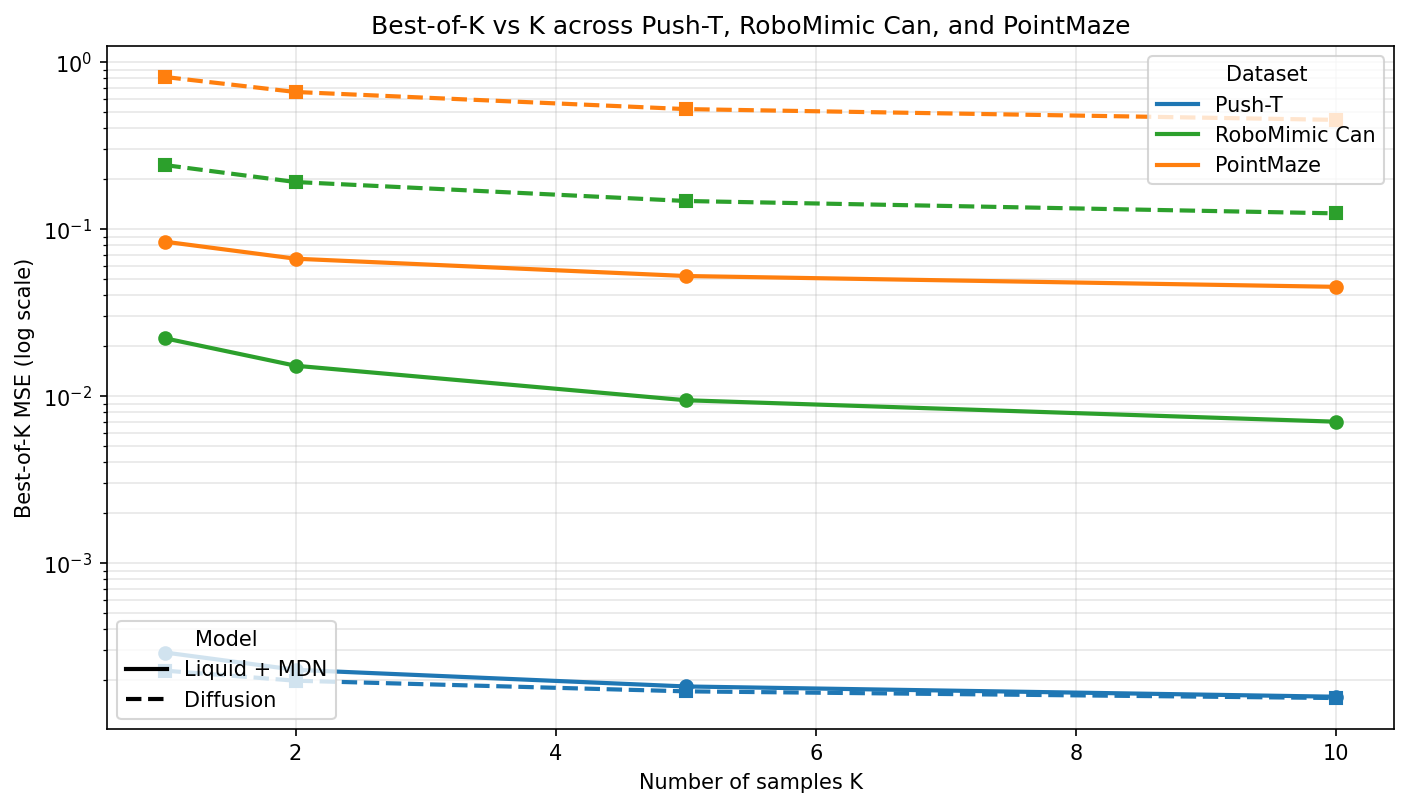
\includegraphics[width=0.95\linewidth]{best_of_k_curve_pusht_vs_robomimic_can_vs_pointmaze_fair_halfparam_deterministic_clip_120epochs.png}
    \caption{Best-of-$K$ MSE across all three datasets. The liquid advantage persists across sample budgets: at $K=10$, liquid models outperform diffusion by $2.4$--$2.5\times$.}
    \label{fig:bestofk-all}
\end{figure*}

\begin{figure*}[!htb]
    \centering
    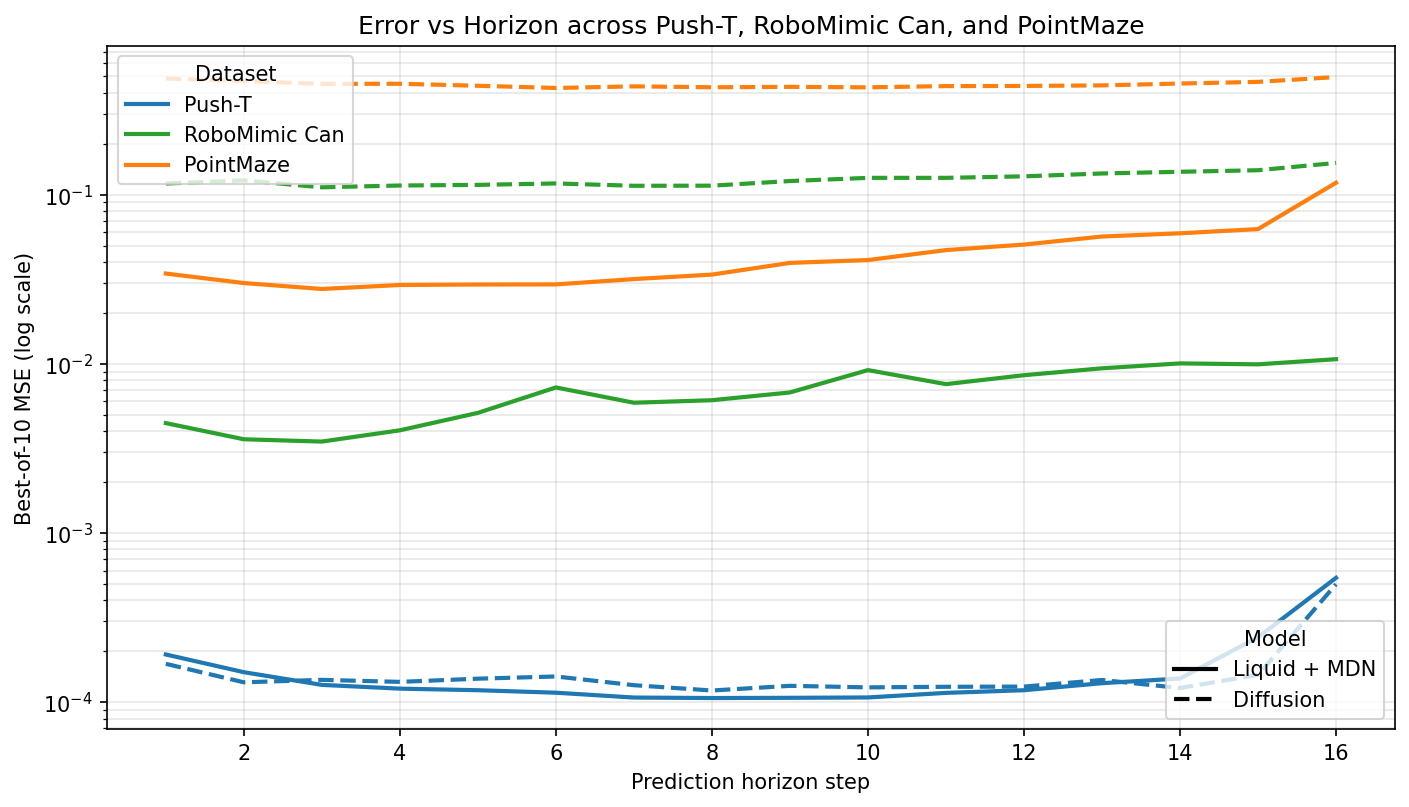
\includegraphics[width=0.95\linewidth]{error_vs_horizon_pusht_vs_robomimic_can_vs_pointmaze_fair_halfparam_deterministic_clip_120epochs.png}
    \caption{Per-horizon error analysis across tasks. All models show increasing error toward the end of the 16-step horizon. The liquid head maintains lower per-step error on all three tasks.}
    \label{fig:horizon-all}
\end{figure*}

\begin{figure*}[!htb]
    \centering
    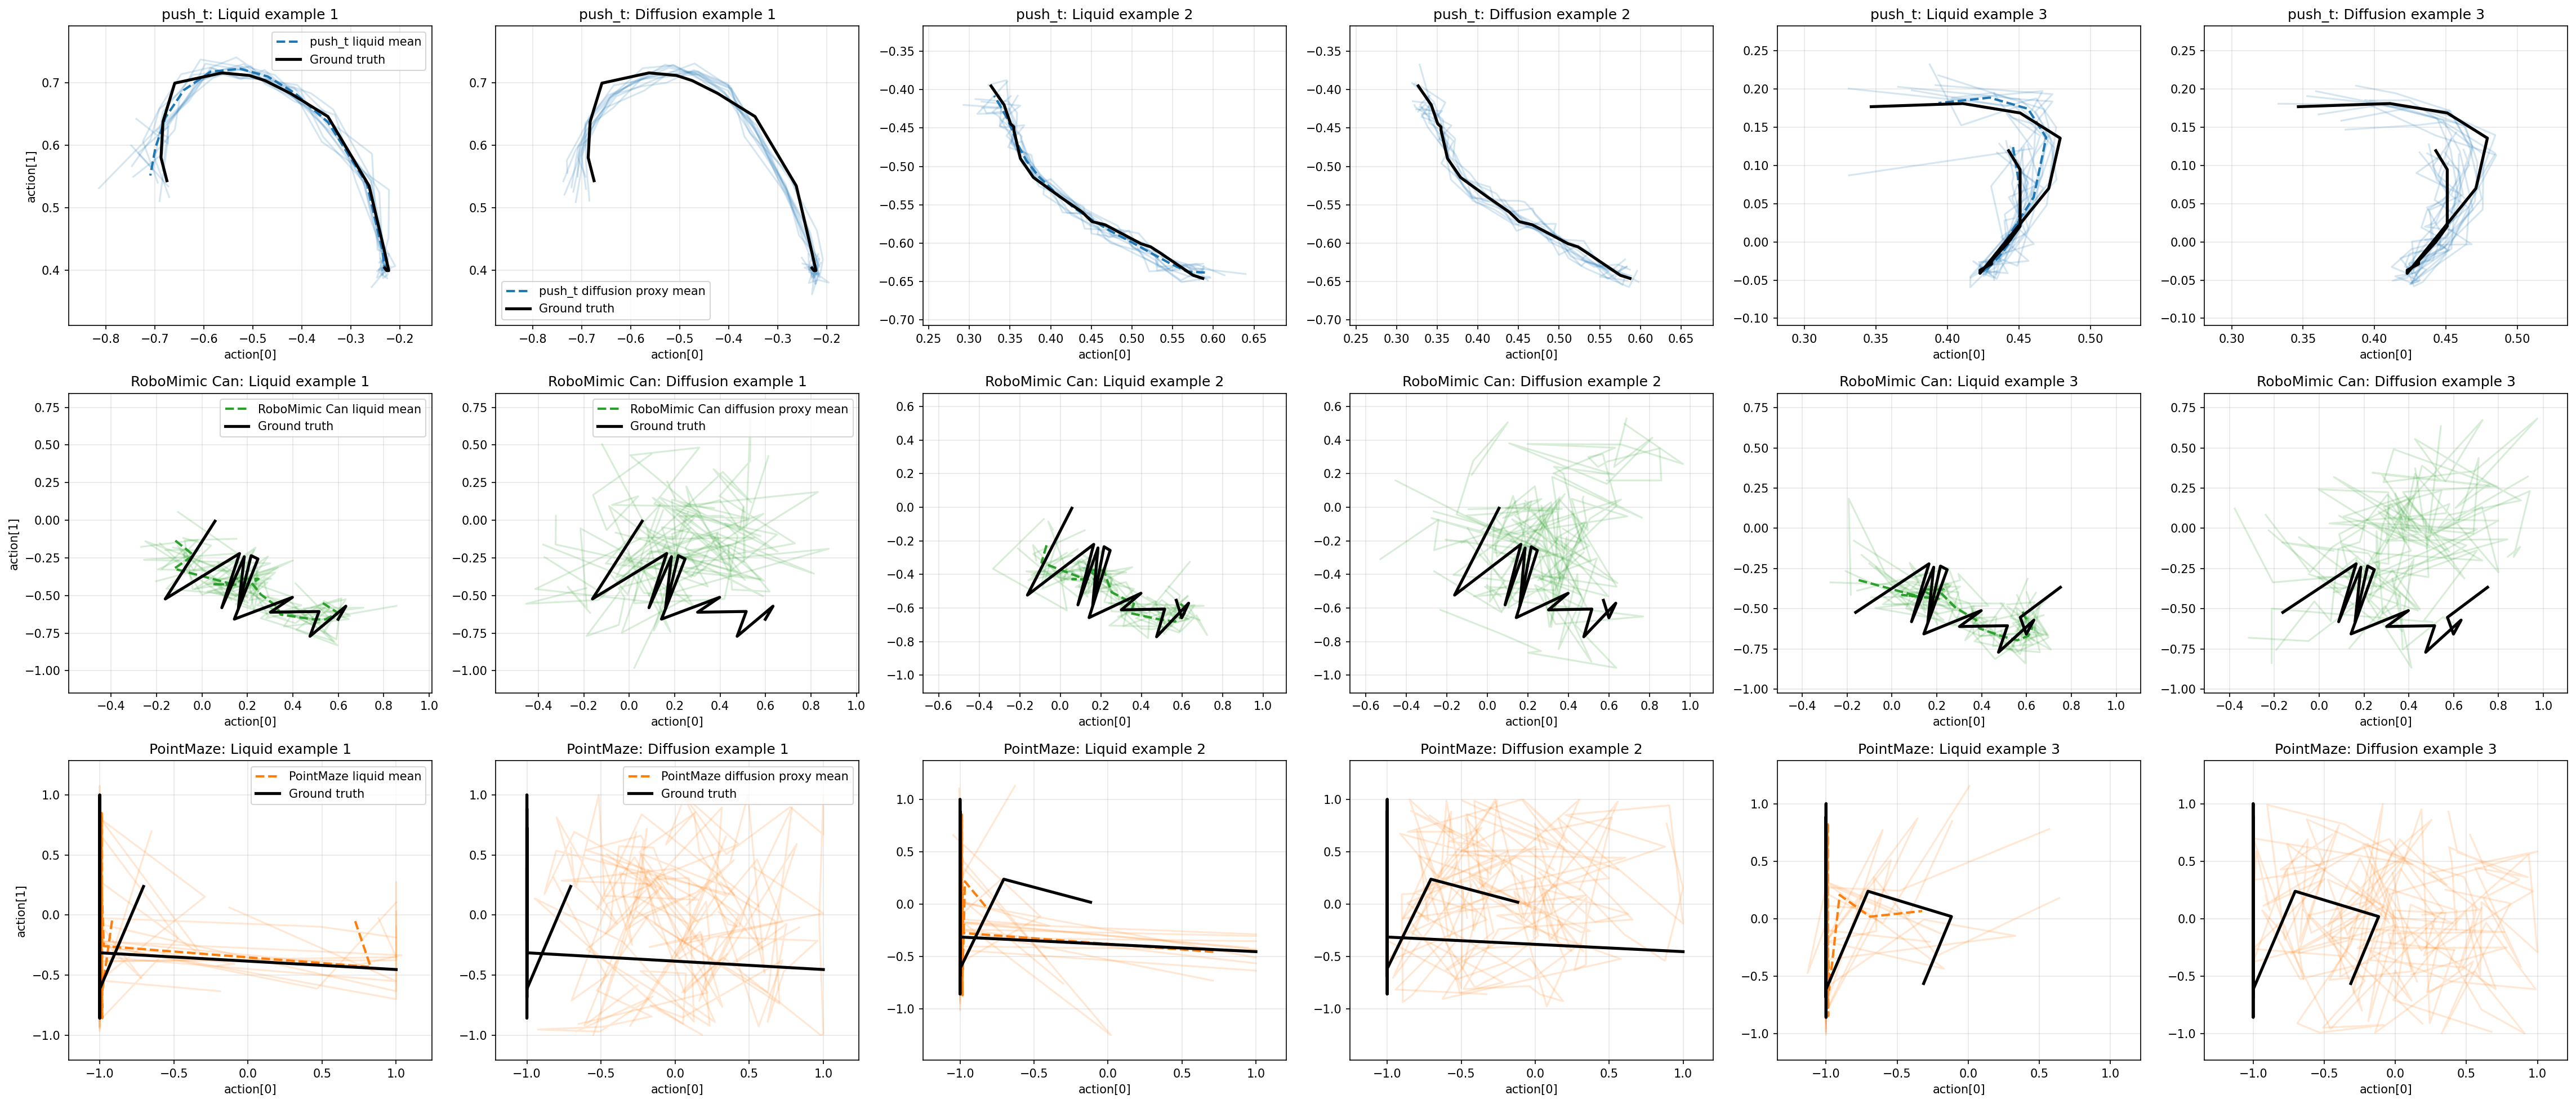
\includegraphics[width=0.95\linewidth]{qualitative_trajectory_samples_pusht_vs_robomimic_can_vs_pointmaze_fair_halfparam_deterministic_clip_120epochs.png}
    \caption{Qualitative sampled trajectories across all tasks. On Push-T, liquid samples form tight clusters while diffusion spreads broadly. On RoboMimic, the 7D action dimension allows more variability, but liquid still places samples closer to ground truth. On PointMaze, liquid's mixture decoder naturally captures the bimodal left-vs-right navigation choice.}
    \label{fig:qualitative-all}
\end{figure*}

\begin{figure*}[!htb]
    \centering
    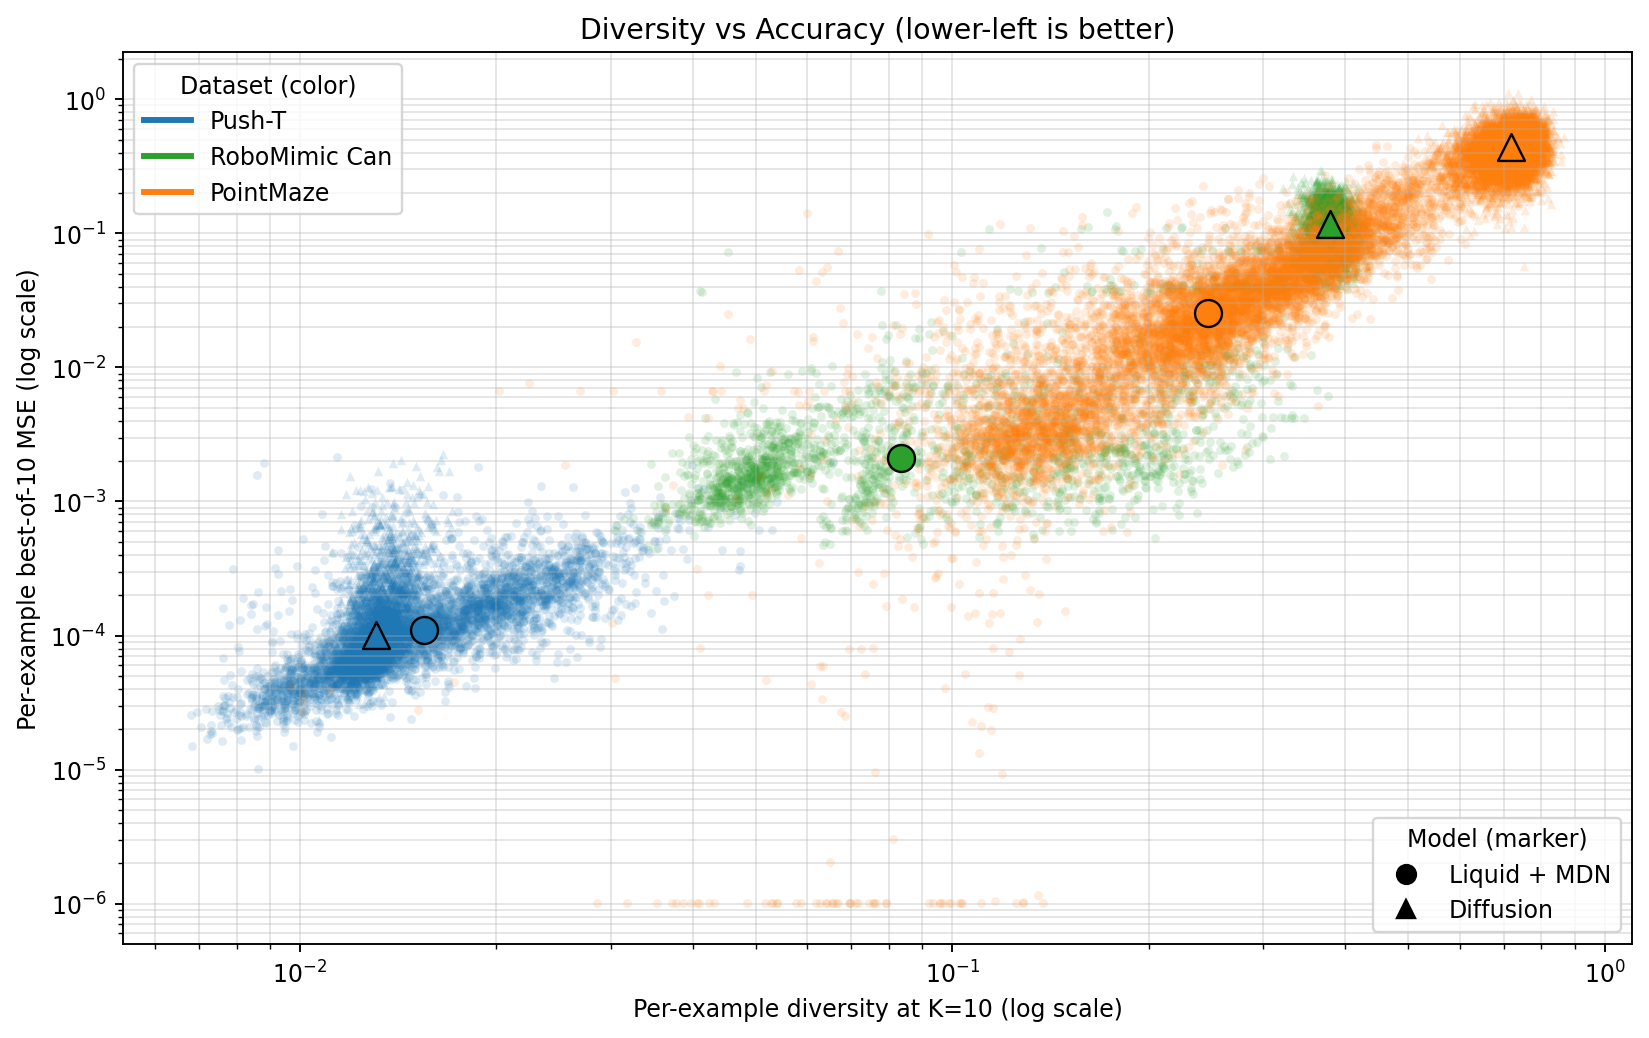
\includegraphics[width=0.95\linewidth]{diversity_vs_error_pusht_vs_robomimic_can_vs_pointmaze_fair_halfparam_deterministic_clip_120epochs.png}
    \caption{Diversity--accuracy trade-off across all tasks (color = dataset, marker = model). Each point corresponds to one evaluation example using $K{=}10$ trajectory samples: the x-axis is sample diversity (spread among sampled trajectories) and the y-axis is best-of-10 MSE (lower is better). The desirable region is lower-left (accurate and diverse enough). Liquid samples (circles) and diffusion samples (triangles) are shown as semi-transparent clouds; large outlined markers denote per-dataset medians to improve readability. Across datasets, liquid tends to achieve lower best-of-10 error at comparable or moderately lower diversity, while diffusion often attains higher diversity but with a higher error floor.}
    \label{fig:diversity-all}
\end{figure*}

\section{Sample Efficiency: Offline Performance vs.\ Training Data Fraction}\label{app:sampleeff-curves}

Figure~\ref{fig:sampleeff-curves} shows per-epoch validation NLL learning curves for every training-data fraction used in the sample-efficiency study of Section~6.2.

\begin{figure}[!htb]
    \centering
    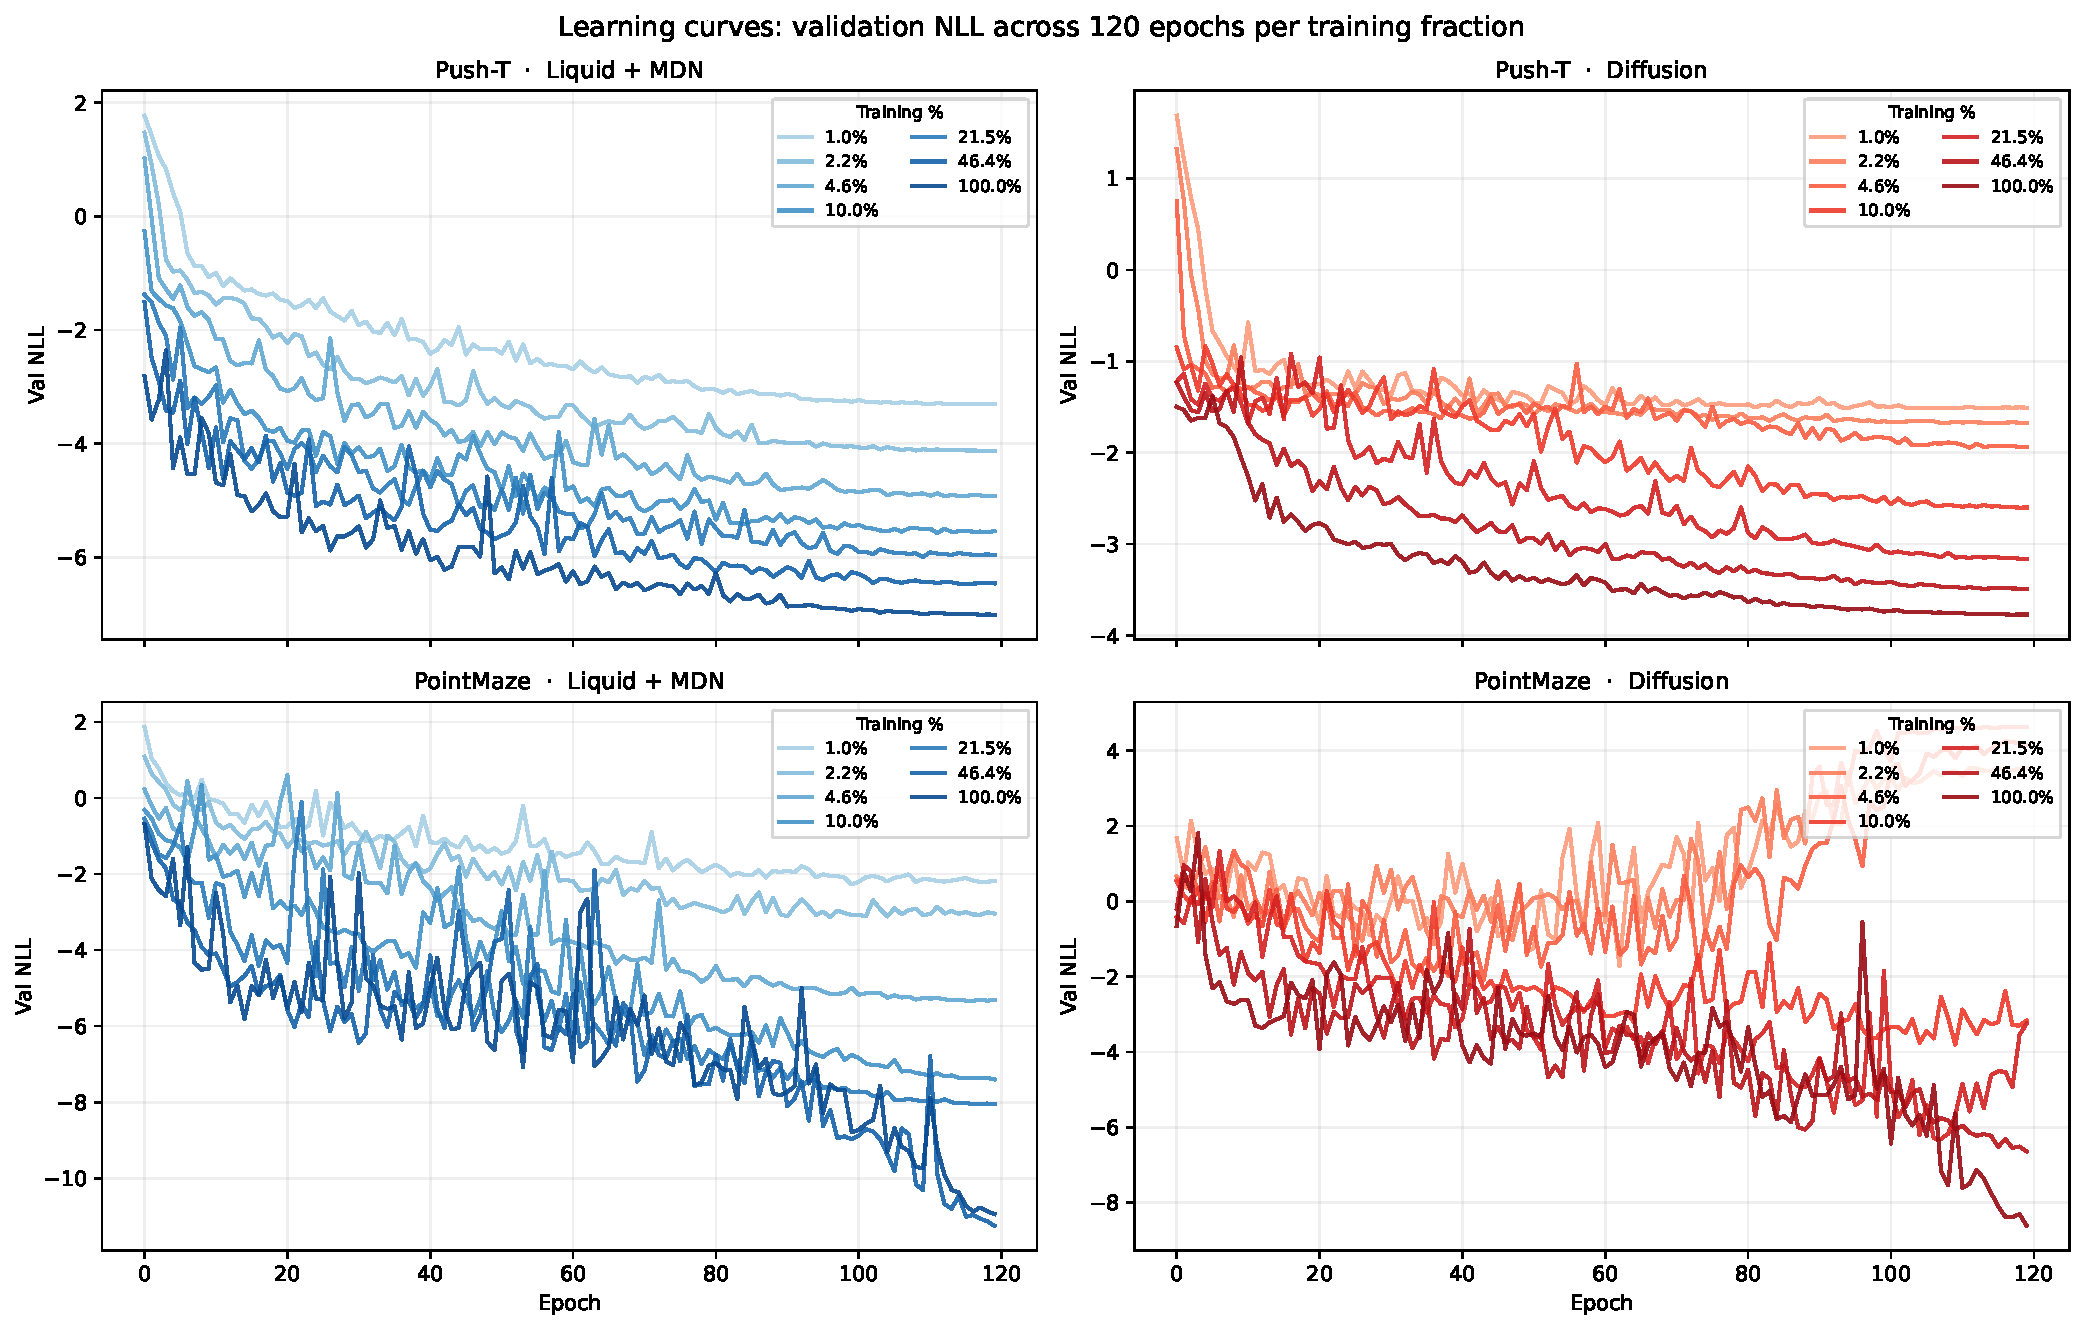
\includegraphics[width=\linewidth]{sample_efficiency_learning_curves.pdf}
    \caption{Validation NLL across 120 training epochs at each training fraction (darker = more data). Liquid curves converge within 20--30 epochs at all data scales; diffusion is slower and noisier at small fractions.}
    \label{fig:sampleeff-curves}
\end{figure}

\section{Theoretical Sample-Efficiency Argument}\label{app:theory}

We provide a compact formalization of why iterative first-order generation incurs a sequential complexity disadvantage relative to continuous-time generator models.

\begin{theorem}[Sequential complexity lower bound for first-order iterative generators]
Let the target trajectory dynamics be Lipschitz, and let a discrete generator produce outputs with first-order updates over $T$ steps. To achieve terminal-state approximation error at most $\epsilon$, the worst-case step complexity satisfies
\begin{equation}
T = \Omega(1/\epsilon).
\end{equation}
\end{theorem}

The statement $T=\Omega(1/\epsilon)$ means that reducing error by one order of magnitude requires (in the worst case) roughly one order of magnitude more sequential refinement steps. For iterative denoising-style generators, this creates a structural compute bottleneck: improved trajectory fidelity is tied to longer step chains, which increases latency and often data requirements because each step-operator must be learned robustly.

\noindent\textit{Proof.} Let $h=1/T$ and consider any explicit first-order one-step iterative generator
\begin{equation}
z_{k+1}=z_k+h\,\phi_h(z_k,k), \qquad k=0,\dots,T-1.
\end{equation}
Under standard consistency assumptions for first-order methods, the local truncation error is $\Theta(h^2)$. With Lipschitz dynamics, stability plus Gr\"onwall's inequality gives global terminal error bounded by
\begin{equation}
\|z_T-\tau(1)\| \le C_1 h = C_1/T
\end{equation}
for some constant $C_1>0$ depending on the Lipschitz constant and horizon. Moreover, this rate is tight in the worst case: there exist smooth Lipschitz systems (including linear systems, cf. the corollary below) for which
\begin{equation}
\|z_T-\tau(1)\| \ge C_0 h = C_0/T
\end{equation}
with $C_0>0$. Therefore, any first-order iterative generator that guarantees terminal error at most $\epsilon$ must satisfy
\begin{equation}
T \ge C_0/\epsilon,
\end{equation}
i.e., $T=\Omega(1/\epsilon)$. \hfill $\square$

Neural ODE-style models (including liquid/CfC-style continuous-time parameterizations) do not inherit this specific first-order iterative-generator lower bound because they learn a shared vector field and then integrate it, rather than learning a distinct correction map for each denoising/refinement step. In practice, this changes the scaling regime: with an order-$p$ integrator, numerical error decreases as $O(h^p)$, so required function evaluations scale like $O(\epsilon^{-1/p})$ (up to constants and adaptivity effects), which is strictly better than $O(1/\epsilon)$ for $p>1$.

\begin{corollary}[Linear-system instantiation]
For $\dot{\tau}(t)=A\tau(t)$ with solution $\tau(1)=e^A\tau_0$, first-order discrete updates satisfy
\begin{equation}
\left\|\left(I+\frac{A}{T}\right)^T-e^A\right\|=\Theta(1/T),
\end{equation}
thus requiring $T=\Omega(1/\epsilon)$ for error $\epsilon$.
\end{corollary}

\section{Stability and Training Practices}

Continuous-time recurrent layers like CfC can suffer from numerical instability if gradients explode during backpropagation through time (BPTT). The following practices ensure stable training.

\paragraph{Gradient clipping.}
We apply $\ell_2$ norm gradient clipping at 1.0 before each optimizer step. This prevents catastrophic updates that can destabilize the recurrent hidden state. For models with $H=960$ hidden dimensions, a norm clip of 1.0 is conservative and rarely triggered, but it provides a safety valve if gradients spike during early training or after data distribution shifts.

\paragraph{Learning rate warm-up.}
We gradually increase the learning rate from 0\% to 100\% of the peak over the first 3 epochs (approximately 8\%--16\% of total training). This ramp-up prevents aggressive parameter updates at the start of training when the model is still learning basic statistics of the action distribution. Once the model has settled into a reasonable solution, full-strength gradient steps help it converge quickly.

\paragraph{Cosine annealing.}
After reaching peak learning rate, we decay via cosine schedule toward a minimum of $3 \times 10^{-7}$. This slow, smooth decay allows the model to continue learning in later epochs without overshooting. The final minimum LR is small enough that the model converges, but non-zero so training does not halt prematurely.

\paragraph{Early stopping disabled.}
We disable early stopping and train for the full 120 epochs. While this seems to contradict standard practice, we find that validation loss on these offline tasks continues to improve throughout training, and checking early checkpoints often yields worse test-time performance. The two-branch training curriculum naturally prevents overfitting; free-running loss acts as a regularizer that keeps the model from memorizing teacher-forced patterns.

\paragraph{Initialization and hyperparameter sensitivity.}
CfC and GRU parameters are initialized from PyTorch defaults (Kaiming uniform for weights, zero for biases). We have found the following to be important for stable convergence.

\paragraph{Hidden size scaling.}
The CfC hidden size should be 1.5--2.0$\times$ the input embedding dimension. In our case, $d_{\mathrm{model}}=512$ and $H_{\mathrm{CfC}}=960$ (1.875$\times$), providing sufficient capacity to model complex temporal dependencies without excessive parameter growth.

\paragraph{Number of CfC layers.}
We use 5 stacked CfC layers in the encoder. Fewer layers (3--4) may undersample the temporal structure; more layers (7+) increase computational cost without proportional accuracy gains on 16-step horizons. Five layers empirically balances expressiveness and efficiency.

\paragraph{GRU decoder initialization.}
The GRU decoder is initialized with hidden size equal to the CfC output size (960). This one-to-one correspondence simplifies the architecture and avoids unnecessary dimension mismatches or projection overhead. The GRU then projects to the mixture density output (5 components $\times$ 3 outputs per component per action dimension) in its linear head.

\paragraph{MDN component count.}
We use $K=5$ mixture components. This is a practical sweet spot: $K=3$ sometimes underfits multimodal tasks like Push-T, while $K=7$ or higher increases computational cost with diminishing accuracy returns. Five components provide enough expressiveness to capture the primary modes of the action distribution without runaway parameter count.

\paragraph{Batch normalization and layer normalization.}
We do not use batch normalization in recurrent layers, as it can interact poorly with BPTT and create subtle gradient flow issues. Instead, the shared transformer backbone (if present) uses layer normalization to stabilize the pre-processed context before it reaches the policy heads. This design cleanly separates:
\begin{itemize}
    \item \textbf{Transformer backbone}: Layer-normalized attention for robust feature extraction,
    \item \textbf{Liquid policy head}: No internal normalization (CfC is inherently normalized via the $V$ and $W$ matrices in the continuous-time ODE),
    \item \textbf{Diffusion policy head}: No internal normalization (diffusion models typically use instance normalization if anything).
\end{itemize}
This separation avoids unexpected interactions while keeping each component's design orthogonal.

\paragraph{Handling different action dimensions.}
The liquid architecture is dimension-agnostic: the GRU decoder outputs a mixture over whatever action dimension is required. For Push-T (3D actions), RoboMimic (7D), and PointMaze (2D), the same architecture template scales without modification. The only change is the final output size of the MDN head ($K \times (3 + d_{\mathrm{action}})$ parameters for mean, log-variance, and logit across the action dimension).

\section{Experimental Setup Details}

\paragraph{Dataset preprocessing and windowing.}
All three datasets are preprocessed into fixed-length 16-step action windows:
\begin{itemize}
    \item \textbf{Push-T}: 24,208 windows total (16,945 train / 3,631 val / 3,632 test),
    \item \textbf{RoboMimic Can}: 72,552 windows (52,230 train / 10,161 val / 10,161 test),
    \item \textbf{PointMaze}: 72,551 windows (50,785 train / 10,883 val / 10,883 test).
\end{itemize}
Each window includes the 16-frame observation history (or low-dimensional state) and the 16 actions to predict.

\paragraph{Action normalization.}
Actions are normalized to zero-mean, unit-variance using dataset statistics before training. This normalization improves the numerical stability of the mixture decoder and allows the model to operate on a consistent scale regardless of the raw action magnitudes (e.g., $\pm 1$ for Push-T vs $\pm 2$ for RoboMimic). At test time, predictions are denormalized back to the original action scale.

\paragraph{Train / validation / test splits.}
Splits are deterministic and stratified by trajectory. We use PyTorch's DataLoader with \texttt{num\_workers=4} and \texttt{pin\_memory=True} for efficient multi-process data loading. Batch size is 64 for all experiments, chosen to balance memory usage and gradient estimation quality.

\paragraph{Reproducibility.}
All experiments use a fixed random seed (42) for PyTorch, NumPy, and Python's built-in random module. The experiment tag \texttt{fair\_halfparam\_deterministic\_clip\_120epochs} encodes the key settings: fair comparison (same context for both heads), half-parameter liquid vs full-parameter diffusion, deterministic evaluation (no stochastic dropout at test time), action clipping enabled, and 120 training epochs. This tag is used throughout the artifact to ensure all logged metrics correspond to the same configuration.

\bibliography{references}

\end{document}

